\documentclass[10pt]{article}

\usepackage{fullpage}
\usepackage{longtable}
\usepackage[pdftex]{graphicx}
\DeclareGraphicsExtensions{.pdf,.jpg}

% no numbers, etc
\pagestyle{empty}

\begin{document}

{\bf Homework 2} \hfill {\raggedleft Thomas Torsney-Weir}

%Each homework problem goes here
\begin{enumerate}
\item % Search
  \begin{enumerate}
  \item % hill climbing
    The biggest issue with using hill climbing is the lack of evaluation
    function.  At best the function would return one if none of the 
    constraints were violated or zero if any were.  Every possible 
    permutation would evaluate to one or zero if it did or didn't satisfy
    all the constraints respectively.  The entire search space would be a
    plateau so the algorithm would just start on a random walk.  We could 
    also get into an infinite loop since hill-climbing doesn't keep track 
    of where it has been.  We may just end up swapping the first two 
    elements over and over again.
    
    A far better solution would be to formulate the problem as a constraint
    satisfaction problem.  Each cell would be a variable and the domain would
    be the ordering, so the first cell would be 1, the second 2, etc.  We 
    would specify constraints like a robotic cell cannot attach a power cord 
    to an appliance until the wiring is complete as $PC<WC$, for example.
    This is a much better solution since we don't really care about finding
    the most efficient line we just care about finding one that works.
  \item % food
    \begin{description}
    \item[Variables] One for each day of the week ($U$ is sunday): 
                     $\{W,T,F,S,U\}$
    \item[Domain] Entrees: $\{VP, GS, PSS, PL, CP\}$
    \item[Constraints] 
      \begin{eqnarray*}
        F & \neq & SF \\
        S & \in & \{PSS, VP\} \\ 
        U & \in & \{PSS, VP\} \\
        (W,T) & \neq & (VP,PL) \\ 
        (T,F) & \neq & (VP,PL) \\
        (F,S) & \neq & (VP,PL) \\
        (S,U) & \neq & (VP,PL) \\
        (W,T,F) & \notin & \{(GS, VP, VP), (GS, VP, GS), 
                             (GS, VP, PSS), (GS, VP, PL), \\
                &        &   (GS, GS, VP), (GS, GS, PSS), 
                             (GS, GS, PL), (GS, PSS, VP) \\
                &        &   (GS, PSS, GS), (GS, PSS, PSS), 
                             (GS, PSS, PL), (GS, PL, VP), \\
                &        &   (GS, PL, GS), (GS, PL, PSS), (GS, PL, PL)\} \\
        (T,F,S) & \notin & \{(GS, VP, VP), (GS, VP, GS), 
                             (GS, VP, PSS), (GS, VP, PL), \\
                &        &   (GS, GS, VP), (GS, GS, PSS), 
                             (GS, GS, PL), (GS, PSS, VP), \\
                &        &   (GS, PSS, GS), (GS, PSS, PSS), 
                             (GS, PSS, PL), (GS, PL, VP), \\
                &        &   (GS, PL, GS), (GS, PL, PSS), (GS, PL, PL)\} \\
        (F,S,U) & \notin & \{(GS, VP, VP), (GS, VP, GS), 
                             (GS, VP, PSS), (GS, VP, PL), \\
                &        &   (GS, GS, VP), (GS, GS, PSS), 
                             (GS, GS, PL), (GS, PSS, VP), \\
                &        &   (GS, PSS, GS), (GS, PSS, PSS), 
                             (GS, PSS, PL), (GS, PL, VP), \\
                &        &   (GS, PL, GS), (GS, PL, PSS), (GS, PL, PL)\} 
      \end{eqnarray*}
    \end{description}
  \end{enumerate}
\pagebreak
\item % CSP
  \begin{enumerate}
  \item % search tree
    \ \\
    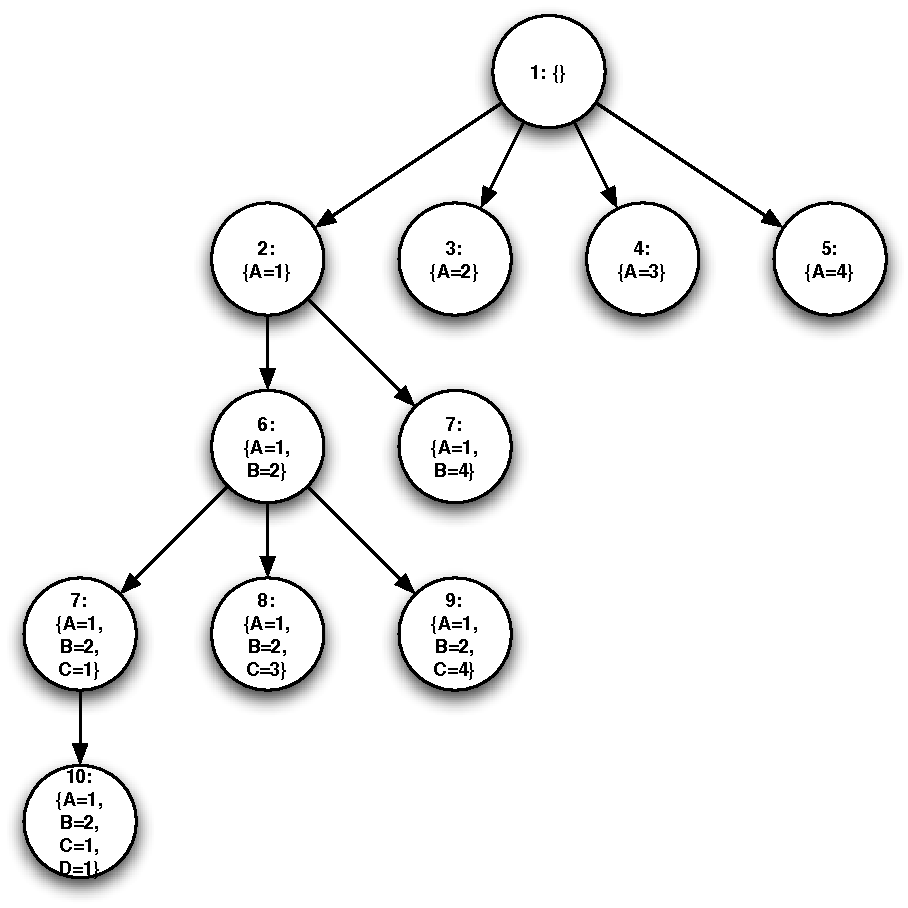
\includegraphics[width=5.5in]{2a_csp_tree.pdf}
  \item % helpful
    \begin{description}
    \item[Most constrained variable]
      This would have allowed us to start by assigning E the value 1 since
      it must be the least value.
    \item[Most constraining variable]
      This will allow us to first choose B when given the choice between B
      and C as B constrains A, C, D, and E.
      This will greatly help to reduce the search space.
    \item[Least constraining variable]
      This would be helpful in choosing a value for A.  This would allow us
      to never try and pick a value for A that would force the value for B
      to be 3.
    \end{description}
  \item % forward chaining
    \begin{tabular}[t]{|c|c|c|c|c|c|}
    \hline 
    Current 
    Assignment & Domain A & Domain B & Domain C & Domain D & Domain E \\
    \hline \hline 
    $A = 1$    & $\{1\}$  & $\{2,4\}$& $\{\}$   & $\{1\}$  & $\{\}$ \\
    \hline 
    $A = 2$    & $\{2\}$  & $\{4\}$  & $\{1\}$   & $\{2\}$ & $\{\}$ \\
    \hline 
    $A = 3$    & $\{3\}$  & $\{2,4\}$& $\{1\}$   & $\{3\}$ & $\{\}$ \\
    \hline 
    $A = 4$    & $\{4\}$  & $\{1,2\}$& $\{1,3\}$ & $\{4\}$ & $\{1,2,3\}$ \\
    \hline 
    $B = 1$    & $\{4\}$  & $\{1\}$  & $\{3\}$   & $\{4\}$ & $\{\}$ \\
    \hline 
    $B = 2$    & $\{4\}$  & $\{2\}$  & $\{1,3\}$ & $\{4\}$ & $\{1\}$ \\
    \hline 
    $C = 1$    & $\{4\}$  & $\{2\}$  & $\{1\}$   & $\{4\}$ & $\{\}$ \\
    \hline 
    $C = 3$    & $\{4\}$  & $\{2\}$  & $\{3\}$   & $\{4\}$ & $\{1\}$ \\
    \hline 
    \end{tabular}
  \end{enumerate}
\pagebreak
\item % adversarial search
  \ \\
  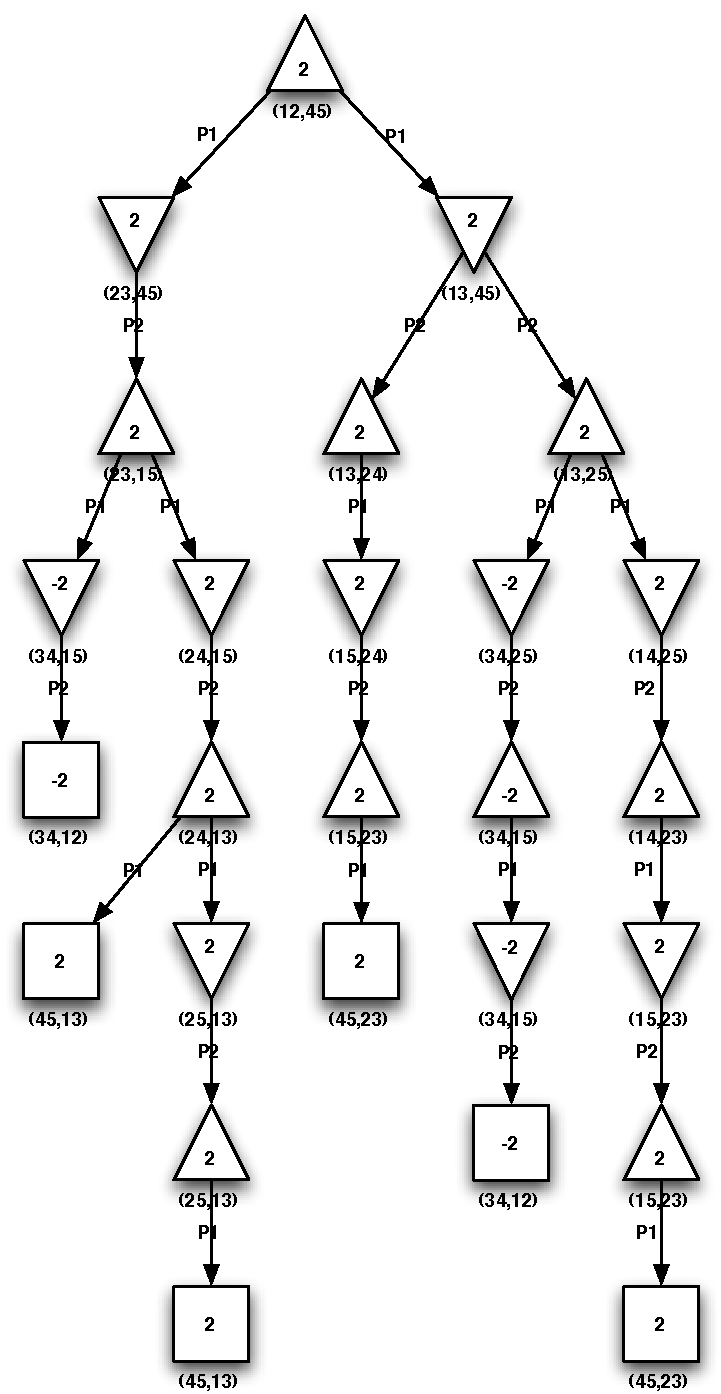
\includegraphics[height=8in]{3_gamesearch.pdf}
\pagebreak
\item % logic
  \begin{enumerate}
  \item 
    \begin{itemize}
    \item $(ST \land C) \lor (C \land CK)$
    \item $CK \Rightarrow D$
    \item $D \Rightarrow ST$
    \item $ST \land C \Rightarrow CH$
    \item $CH$
    \end{itemize}
  \item
    \begin{itemize}
    \item $C \land (ST \lor CK)$
    \item $\lnot CK \lor D$
    \item $\lnot D \lor ST$
    \item $\lnot ST \lor \lnot C \lor CH$
    \item $CH$
    \end{itemize}
  \item % resolution
    \ \\
    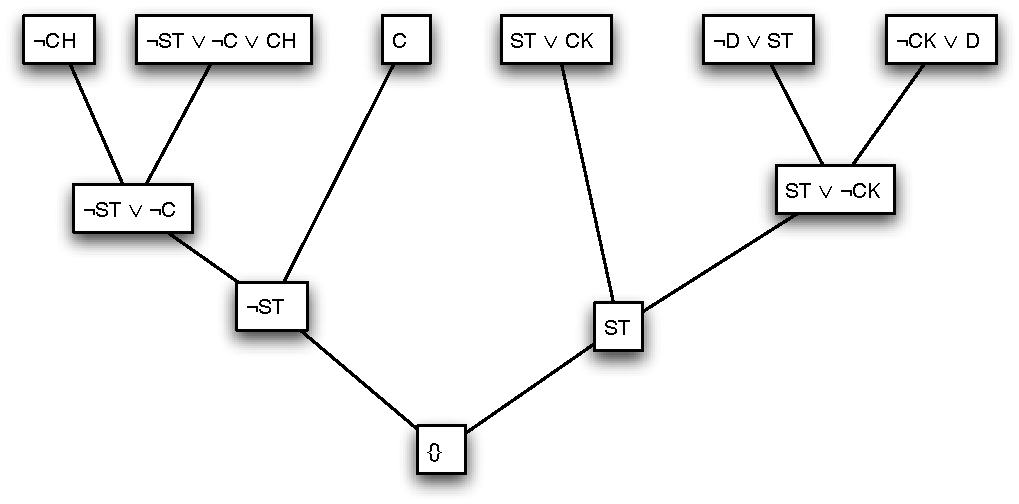
\includegraphics[width=5.5in]{4c_proof.pdf}
  \item % FOL
    \begin{itemize}
    \item $(LIKES(I, C) \land HAS(I, ST)) \lor (LIKES(I,C) \land LIKES(I,CK))$
    \item $LIKES(I,CK) \Rightarrow LIKES(I,D)$
    \item $LIKES(I,D) \Rightarrow HAS(I,ST)$
    \item $HAS(I,ST) \land LIKES(I,C) \Rightarrow IS(I,CH)$
    \item $IS(I,CH)$
    \end{itemize}
  \item % variation
    \begin{itemize}
    \item $\forall x, IS(x, PERSON) \land 
                      ((LIKES(x, C) \land HAS(x, ST)) \lor 
                       (LIKES(x,C) \land LIKES(x,CK)))$
    \item $\forall x, IS(x, PERSON) \land LIKES(x,CK) \Rightarrow LIKES(x,D)$
    \item $\forall x, IS(x, PERSON) \land (LIKES(x,D) \Rightarrow HAS(x,ST)$
    \item $\forall x, IS(x, PERSON) \land HAS(x,ST) \land LIKES(x,C) 
                      \Rightarrow IS(x,CH)$
    \item $\forall x, IS(x, PERSON) \Rightarrow IS(x,CH)$
    \end{itemize}
  \end{enumerate}
\end{enumerate}

\end{document}

